\documentclass[a4paper]{article}

%% Language and font encodings
\usepackage[english]{babel}
\usepackage[utf8x]{inputenc}
% \usepackage[T1]{fontenc}
\usepackage{float}
\usepackage{url}

\usepackage{helvet}
\renewcommand{\familydefault}{\sfdefault}

%% Sets page size and margins
\usepackage[a4paper,top=3cm,bottom=2cm,left=3cm,right=3cm,marginparwidth=1.75cm]{geometry}

%% Useful packages
\usepackage{amsmath}
\usepackage{graphicx}
\usepackage[colorinlistoftodos]{todonotes}
\usepackage[colorlinks=true, allcolors=blue]{hyperref}


\usepackage{listings}
\lstset{basicstyle=\ttfamily,
  showstringspaces=false,
  commentstyle=\color{blue},
  keywordstyle=\color{black}
}



\title{Exercise 3: Training End-to-end driving networks}
\author{Michael Floßmann, Kshitij Sirohi, Hendrik Vloet}
\pagestyle{empty}
\begin{document}
\maketitle

\section{Introduction}
\subsection{Goals}
The main objective of this assignment was to reproduce the work done in the
paper by Codevilla et al. \cite{imitation}. This included:
\begin{itemize}
\item Reconstructing the described networks in pytorch (``command input'' and ``branched'')
\item Training the reconstructed networks on the original dataset from
  \cite{imitation} with image augmentations implemented in a previous
  assignment (with some ablation studies).
\item Optional: Implement a recurrent architechture to model the temporal domain.
\end{itemize} 

\subsection{Issues}

During the assignment we encountered several which delayed our development progress. Due to these problems we where not able to achieve the goals above. Below we will state a short list with the most problematic issues, attends to solve them and whether this worked or not. After that, a short list of results we can provide within this report will follow.

	\paragraph{Corrupted files} While reading in the dataset, we encountered OSErrors. This was due to the corruption of one (and sometimes more than one) file. This file was basically empty and we had to write a "CheckCorruption" like routine to scan the dataset beforehand in order to avoid further crashes. Our routine works and removes corrupted files from the training set.
	\paragraph{Disk Space} Disk space was not sufficient to unpack the whole dataset and as consequence we where force to fetch the dataset from the university network which is slower than using the internal SSD (where access was restricted)
	\paragraph{Runtime} Training and Validation are quite time consuming, around 10h to 15h are normal for 5 epochs of training. We tried to speed it up by increasing the number of workers in the pytorch loader and accessing the validation sets in a more sequential way. This reduced the time consumption significantly.
	\paragraph{Nightly Reboots} We wanted to train during the night, but due to the nightly reboots, the training was interrupted. We could do nothing regarding this problem. The only thing we could do was to save the model on a periodic basis and continue after the reboot with a new training run, but the old model.
	
\begin{lstlisting}[language=bash, caption={Nigthly Reboot Interruption}]

25153.85s - Train Epoch: 2 [344800/480640 (72%)]    Loss: 0.006571
25156.82s - Train Epoch: 2 [344900/480640 (72%)]    Loss: 0.006483
25159.51s - Train Epoch: 2 [345000/480640 (72%)]    Loss: 0.026645
25162.00s - Train Epoch: 2 [345100/480640 (72%)]    Loss: 0.019915
                                                                               
*** FINAL System shutdown message from root@login2 ***                       
System going down IMMEDIATELY                                                  
                                                                               
Nightly routine re-boot                                                        
                                                                               
25164.69s - Train Epoch: 2 [345200/480640 (72%)]    Loss: 0.006574
25167.05s - Train Epoch: 2 [345300/480640 (72%)]    Loss: 0.006452
25170.02s - Train Epoch: 2 [345400/480640 (72%)]    Loss: 0.027064
25173.58s - Train Epoch: 2 [345500/480640 (72%)]    Loss: 0.023583
Connection to login.informatik.uni-freiburg.de closed by remote host.
Connection to login.informatik.uni-freiburg.de closed.

\end{lstlisting}

\paragraph{Retain Graph Error} This error occurred two times in total. Both in the way like listed below. After the first time, we did as suggested by the program and set the \textbf{retain\_graph} attribute to true. But it did not help and the error did pop up again. This happened only on one of our private homestations, so we were basically forced to work on the pool computers.

\begin{lstlisting}[language=bash, caption={Nigthly Reboot Interruption}]


2251.09s - Train Epoch: 1 [120000/526080 (23%)]    Loss: 0.041661
2251.59s - Train Epoch: 1 [120050/526080 (23%)]    Loss: 0.039515
2252.20s - Train Epoch: 1 [120100/526080 (23%)]    Loss: 0.037241
2252.68s - Train Epoch: 1 [120150/526080 (23%)]    Loss: 0.035107
Traceback (most recent call last):
  File "./Branched.py", line 401, in <module>
    main()
  File "./Branched.py", line 359, in main
    loss.backward()
  File "/home/hive/pytorch_venv/lib/python3.5
  /site-packages/torch/tensor.py", line 93, in backward
    torch.autograd.backward(self, gradient, retain_graph,
     create_graph)
  File "/home/hive/pytorch_venv/lib/python3.5/site-packages/torch/
  autograd/__init__.py", line 89, in backward
    allow_unreachable=True)  # allow_unreachable flag
RuntimeError: Trying to backward through the graph a second time, 
but the buffers have already been freed. 
Specify retain_graph=True when calling backward the first time.

\end{lstlisting}

\paragraph{Deus Ex Machina} Somebody turns of a pool machine where we are training on.

\section{Results}
We managed to let the network "Command Input" run a training with augmented images and non-augmented images.
The training run with the augmented images is non-complete, since it was interrupted by a nightly reboot.
Settings were the same for both runs:
\begin{itemize}
	\item Batch size: 100
	\item 80\% training, 20\% validation split
	\item Learning Rate 0.0002
	\item Evaluation after every 500 batches
  \end{itemize}

\paragraph{Missing information from the paper} The paper doesn't state several
important hyperparameters like the weights in equation (6) (page 4), or the
magnitudes of the random parameters in the data augmentation. A git issue has
been filed for the weight parameter, but the information given was inconcludive.
(\url{https://github.com/carla-simulator/imitation-learning/issues/19})

\subsection{Results for Command Input: Augmented}
The loss plots are displayed in the figures \ref{fig:augmented_command_train_loss}
and \ref{fig:augmented_command_eval_loss}. The training error is too noisy to
read anything substantial from it and the validation loss doesn't show a clear
trend except for right after the very first validation when the model was
completely untrained.

This may be an effect of the data augmentation hyperparameters not being tuned
correctly, distorting the image too much and making the model underfit.
The errors for the test set are listed in table \ref{tab:error_command_aug}.
\begin{table}[H]
  \centering
  \caption{Error values for augmented command values}
  \begin{tabular}{lcc}
    &Mean squared error& Median squared error \\ \hline
    Steer & 0.0357 & 0.0010 \\
    Gas &0.0879&0.0098
  \end{tabular}
  \label{tab:error_command_aug}
\end{table}
  \begin{figure}[H]
    \centering
    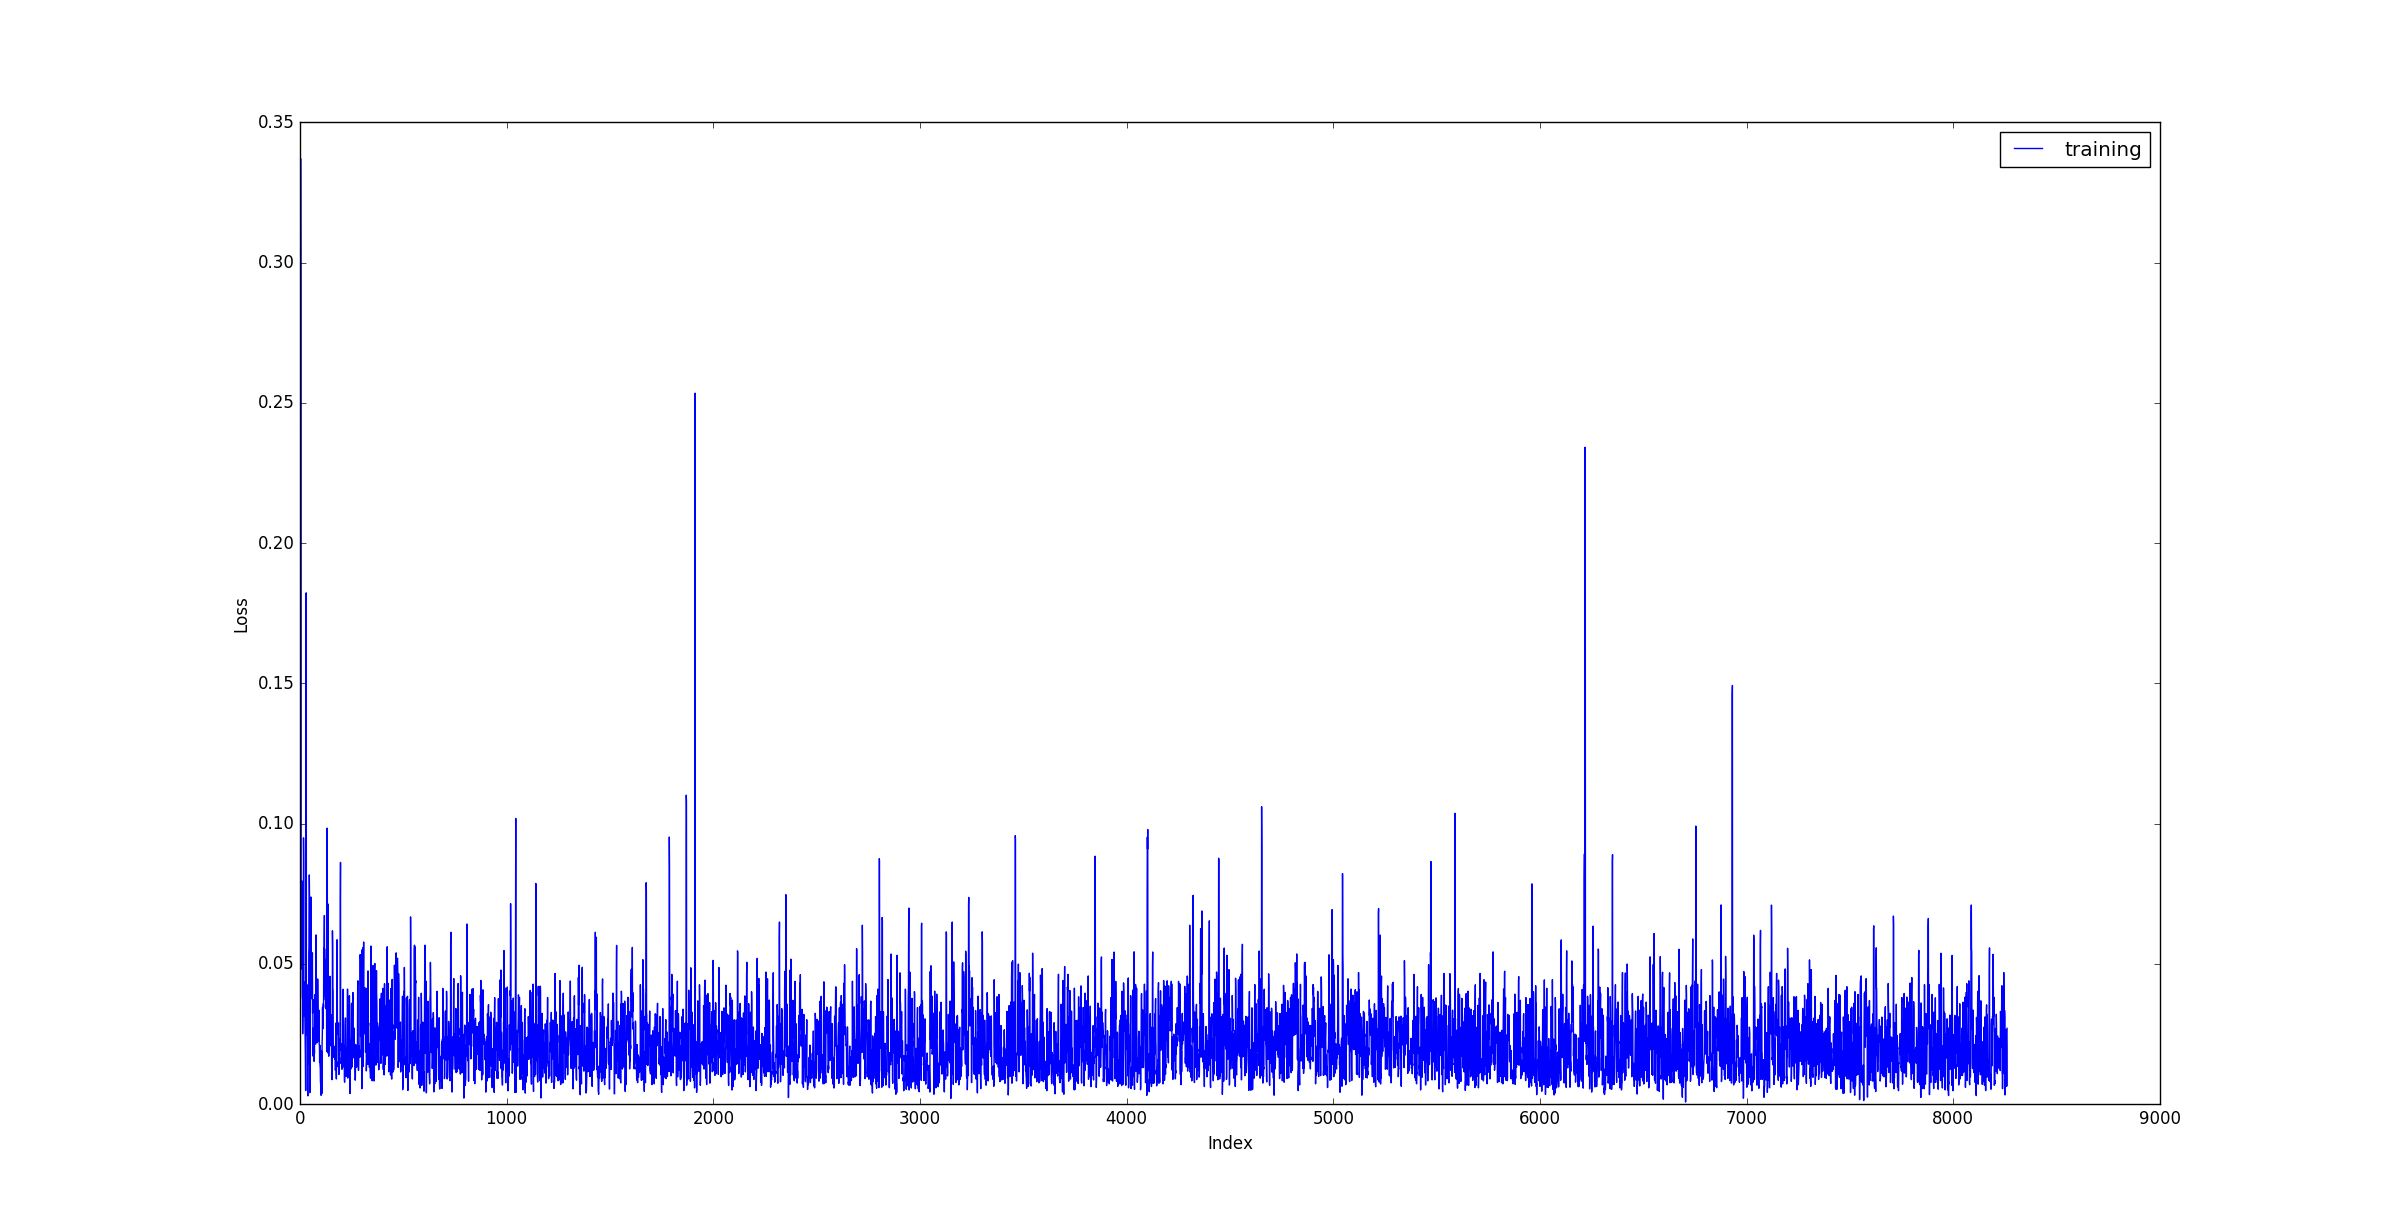
\includegraphics[width=\textwidth, height=8cm]{../pics/command_input_training_augmented.png}
    \caption{Train losses for augmented command input}
    \label{fig:augmented_command_train_loss}
  \end{figure}
%\end{minipage}
%\begin{minipage}{0.45\textwidth}
  \begin{figure}[H]
    \centering
    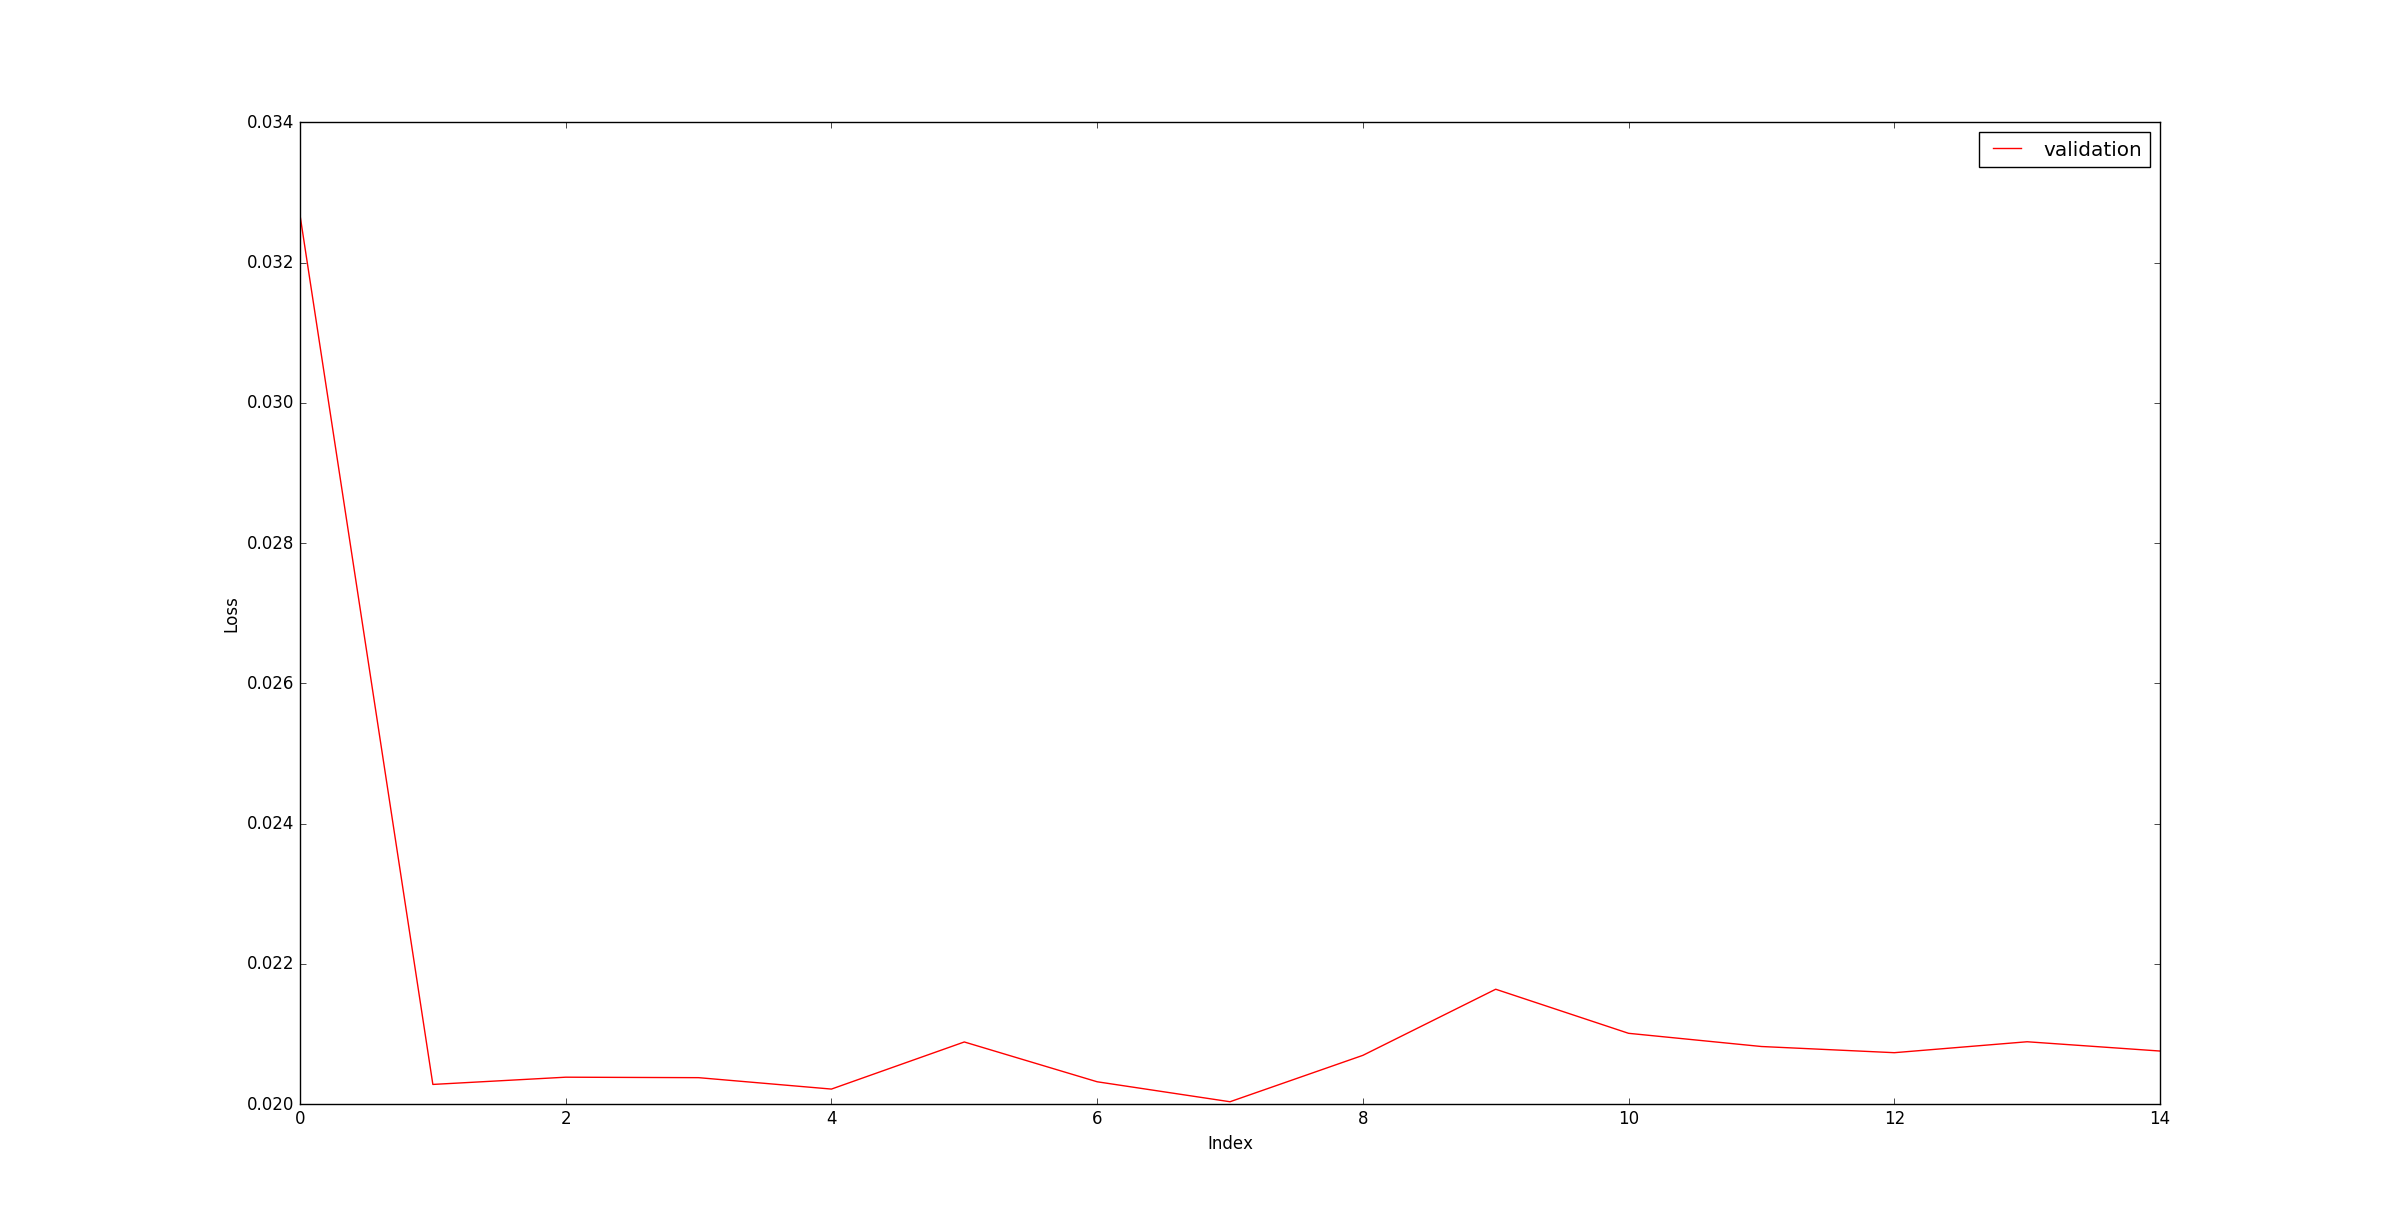
\includegraphics[width=\textwidth, height=8cm]{../pics/command_input_validation_augmented.png}
    
    \caption{Validation losses for augmented command input}
    \label{fig:augmented_command_eval_loss}
  \end{figure}


  \subsection{Command Input: Non-augmented}
  The loss plots are displayed in the figure \ref{fig:non_augmented_train_loss}
  and \ref{fig:non_augmented_val_loss}. While the training error is very noisy
  still, the validation error shows a diminishing trend each epoch. This could
  suggest that more training epochs are needed for proper predictions. Also, the
  visible trend furtherly suggests that for the augmented training the
  augmentation hyperparameters must be better tuned in order not to underfit the
  model.

  The errors for the test set are listed in table \ref{tab:error_command_non_aug}.
\begin{table}[H]
  \centering
  \caption{Error values for non-augmented command values}
  \begin{tabular}{lcc}
    &Mean squared error& Median squared error \\ \hline
    Steer & 0.0357 & 0.0017 \\
    Gas &0.0865&0.0109
  \end{tabular}
  \label{tab:error_command_non_aug}
\end{table}
%\begin{minipage}{0.45\textwidth}
  \begin{figure}[H]
    \centering
    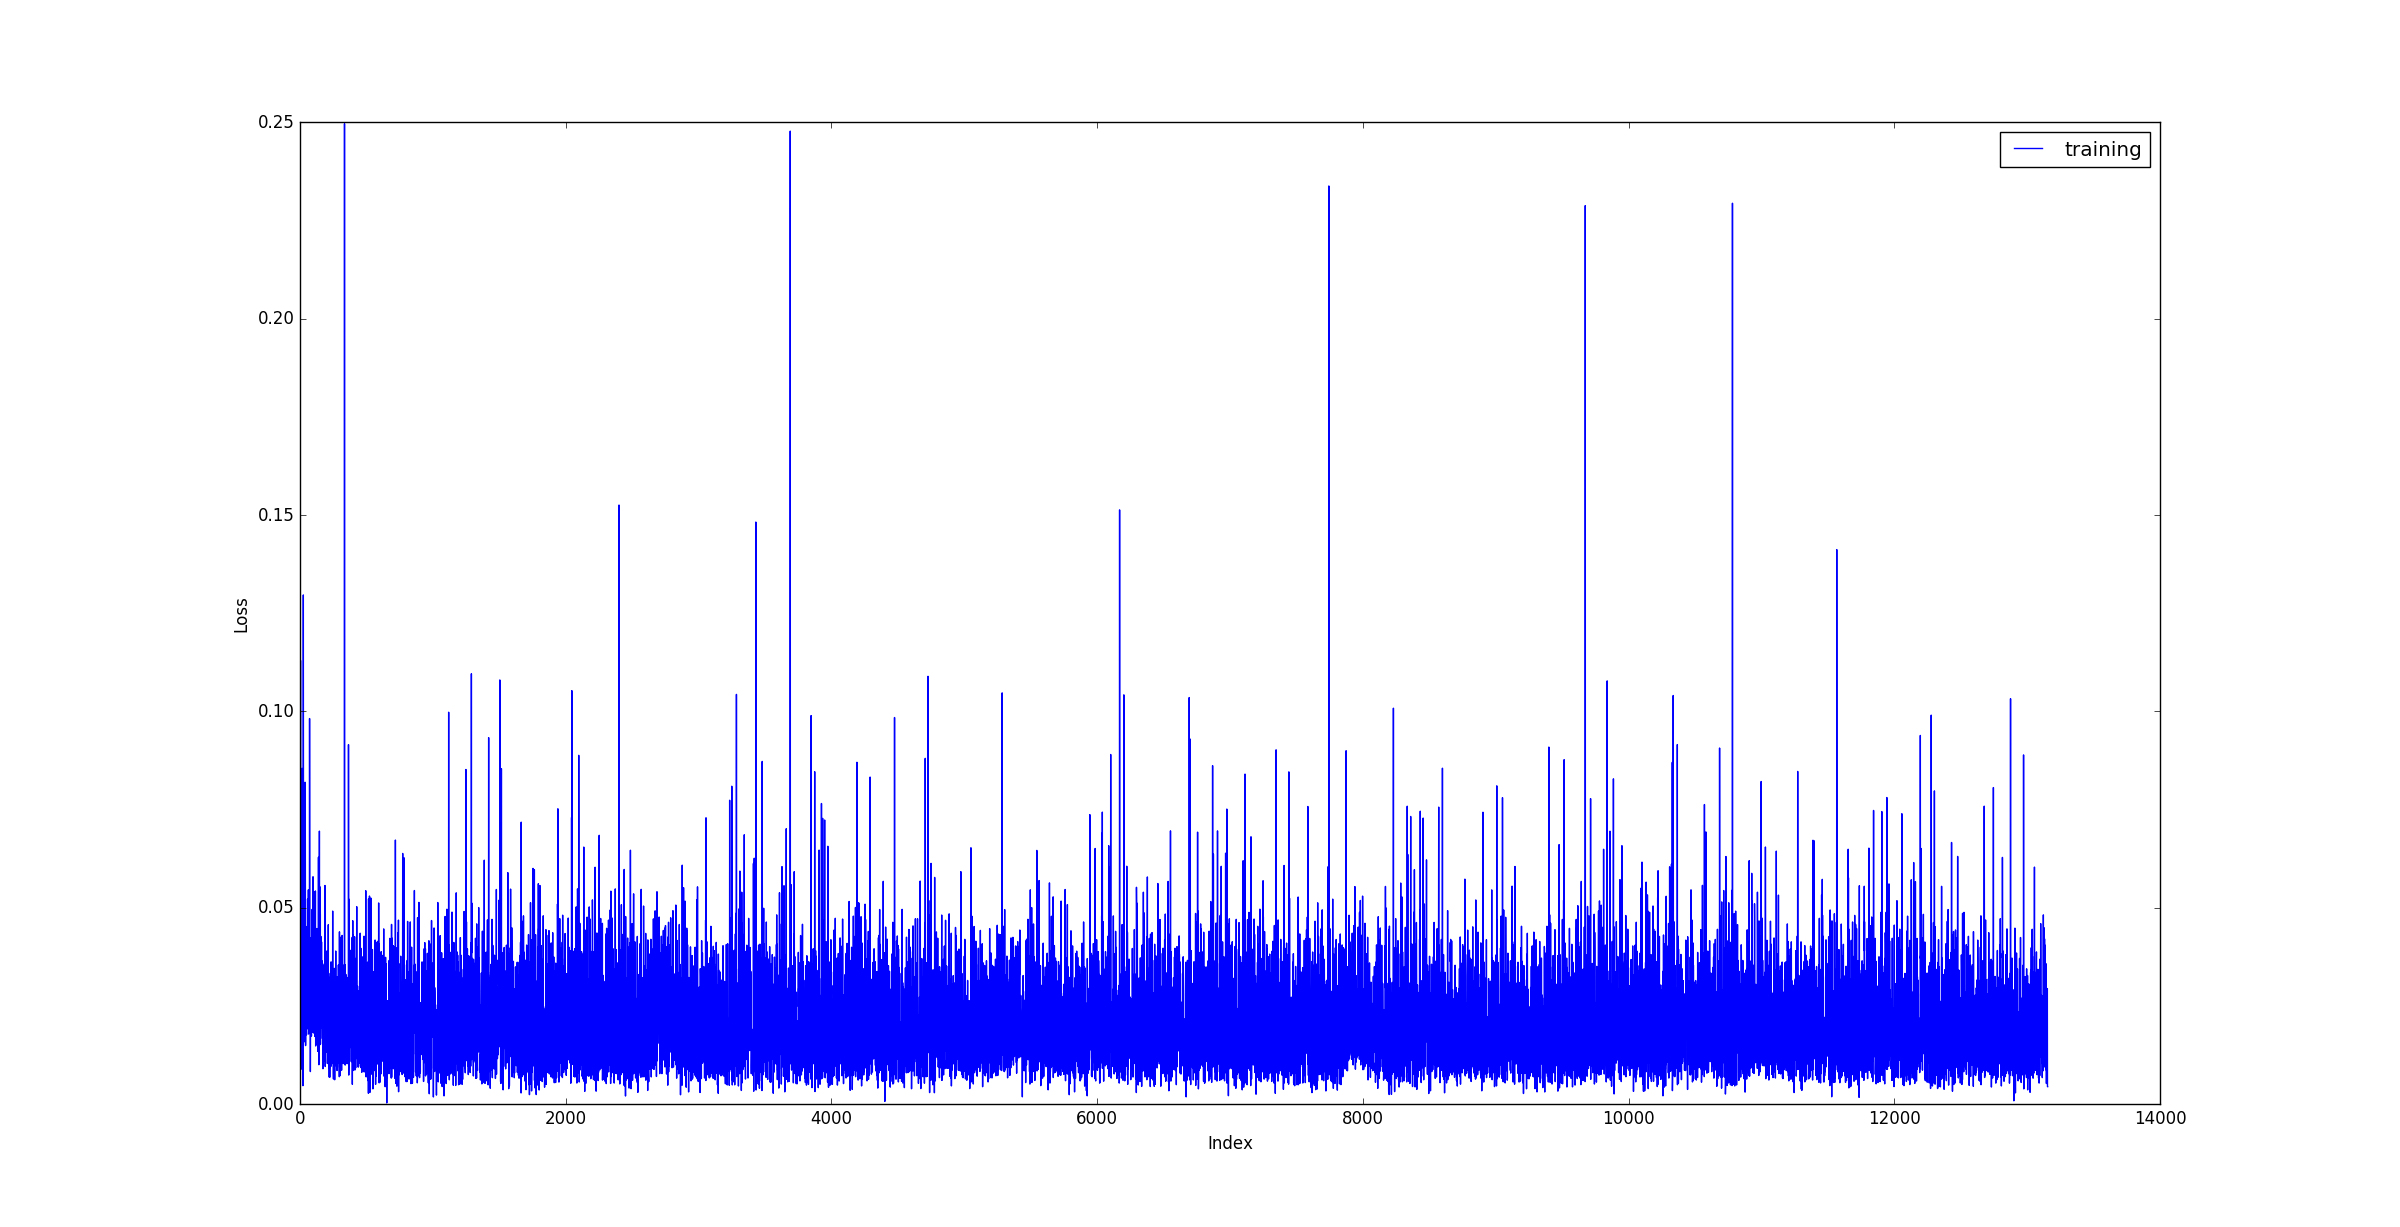
\includegraphics[width=\textwidth, height=8cm]{../pics/command_input_nonaugmented_training.png}
    \caption{Train losses for not augmented command input}
    \label{fig:non_augmented_train_loss}
  \end{figure}

%\end{minipage}
%\begin{minipage}{0.45\textwidth}
  \begin{figure}[H]
    \centering
    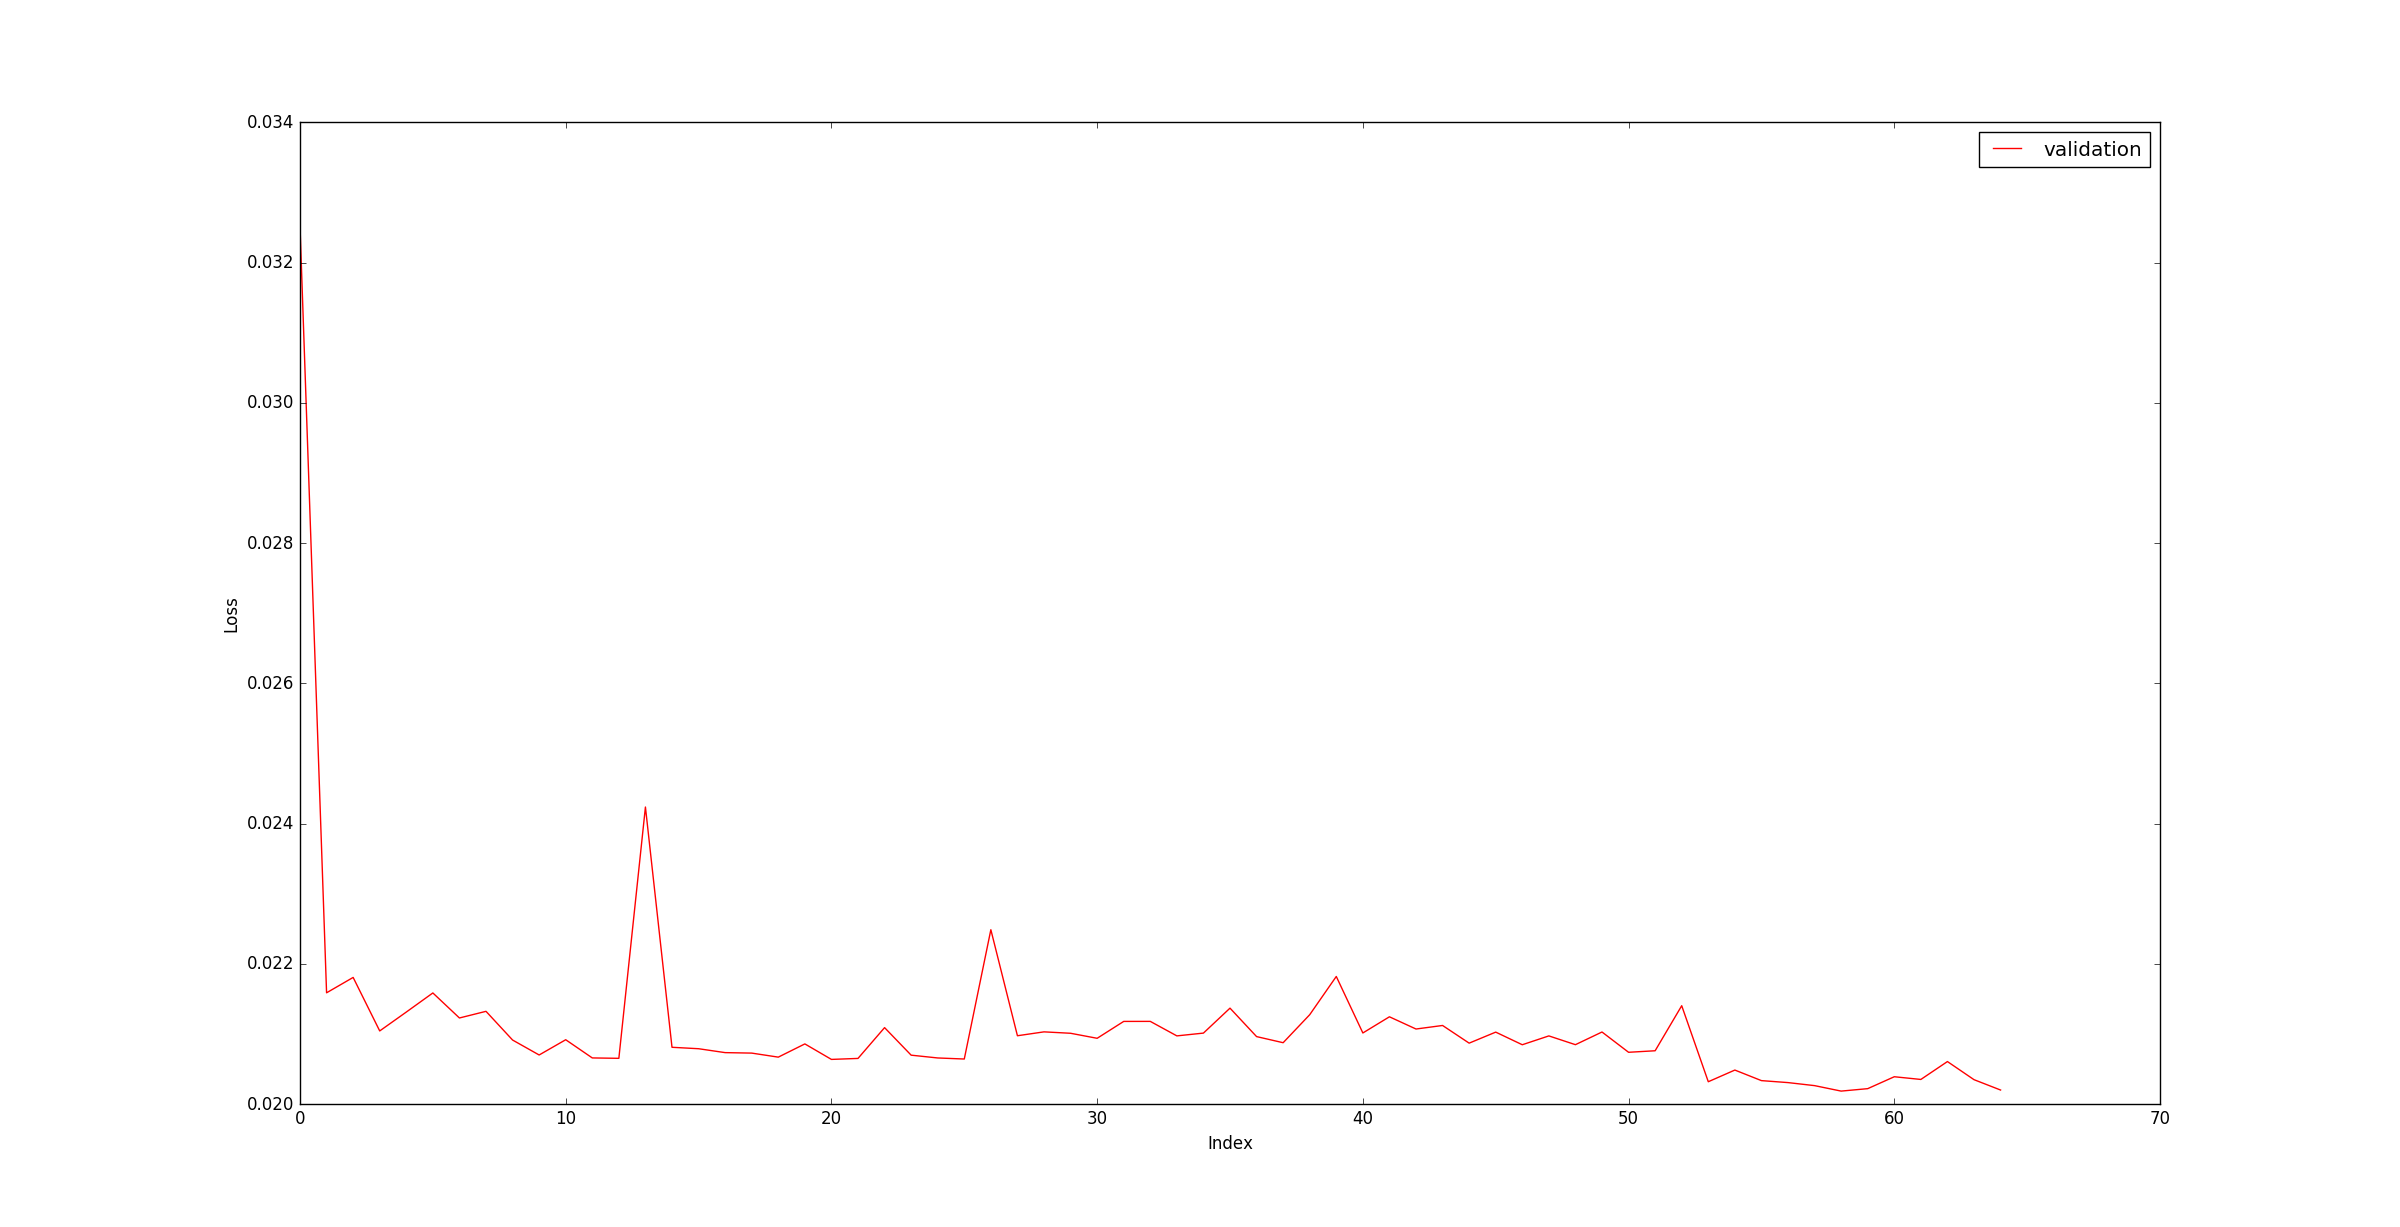
\includegraphics[width=\textwidth, height=8cm]{../pics/command_input_nonaugmented_validation.png}
    \caption{Validation losses for not augmented command input}
    \label{fig:non_augmented_val_loss}
  \end{figure}

  % \end{minipage}

  \subsection{Branched}

The branched could not be analyzed because several issues got in the way. This
will be addressed for the next assignment.

\begin{thebibliography}{9}
\bibitem{imitation}
Codevilla, Felipe and Müller, Matthias and López, Antonio and Koltun, Vladlen
and Dosovitskiy, Alexey.
\textit{End-to-end Driving via Conditional Imitation Learning.}
ICRA 2018
\end{thebibliography}

\end{document}